\subsection{Long-Short-Term-Memory (LSTM)}

An LSTM is a special type of RNN. RNNs use recurrent units to learn temporal features from sequence data, as LSTMs do. However, what happens inside the recurrent unit is very different between the two, as shown in image \vref{fig:lstm}.


\begin{figure}
	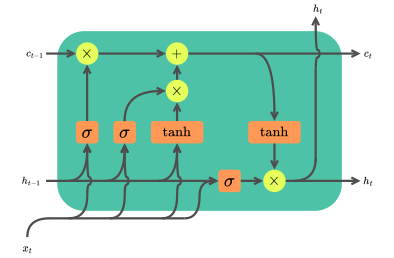
\includegraphics[width=0.5\textwidth]{images/lstm}
	\caption{LSTM unit, source \cite{wiki:lstm}.}
	\label{fig:lstm}
\end{figure}

Assuming we know the basic operation of RNNs, we are going to describe the operation of an LSTM layer at time $t$, to which comes the time sequence $x_1, x_2, \cdots, x_T$:

\begin{description}
	\item[Hidden state and input]: the hidden state of a previous time step $h_{t-1}$ and the input of the current time step $x_t$ are combined before running copies through various operational gates using concatenation between vectors.
	$$
	\left[h_{t-1} \mid x_{t}\right]
	$$
	\item[Cell state:] $c_{t-1}$ is a recurrent input representing the long-term memory of the network. In fact, it will be modified only slightly by the current time step with a sequence of linear additions and Hadamard products (component-wise), resulting in the next cell state $c_t$.
	\item[Forget gate:] this gate controls what saved information should be forgotten, and consists of a simple sigmoid neural network layer that multiplies the previous result with a weight matrix $W_f$, adds a bias vector $b_f$ and gives the result as input to a sigmoid activation function. As the sigmoid function varies between 0 and 1, it determines which cell state values should be discarded (multiplied by 0), remembered (multiplied by 1) or partially remembered (multiplied by a value between 0 and 1).
	$$
	f_{t}=\sigma\left(W_{f} \cdot\left[h_{t-1} \mid x_{t}\right]+b_{f}\right)
	$$
	\item[Input gate:] consists of a sigmoid neural layer, which multiplies [$h_{t-1} | x_t$] with a weight matrix $W_i$, adds a bias $b_i$ and gives the result as input to a sigmoid function. Outputs between 0 and 1 identify the important elements of [$h_{t-1} | x_t$] that are to be added to the cell state $c_{t-1}$.
	\item[Proposed update cell state]: consists of a $\tanh$ neural layer, which multiplies [$h_{t-1} | x_t$] with a weight a matrix $W_c$, adds a bias vector $b_c$ and gives the result as input to the activation function $\tanh$. The output $\tilde{c}_t$ determines the candidate values for storage within the cell state.
	$$
	\tilde{c}_{t}=\tanh \left(W_{c} \cdot\left[h_{t-1} \mid x_{t}\right]+b_{c}\right)
	$$
	\item[Update cell state:] the previous cell state $c_{t-1}$ is multiplied by the result of forget gate $f_t$ to remove irrelevant information, and the result is added component by component to the vector of candidate values $\tilde{c}_{t}$, weighted by the output of input gate $i_t$, to finally obtain the next cell state $c_t$.
	$$
	c_{t}=f_{t} \odot c_{t-1}+i_{t} \odot \tilde{c}_{t}
	$$
	\item[Output gate:] consists of a simple sigmoid neural layer that, again, multiplies [$h_{t-1} | x_t$] with a weight matrix $W_o$, adds a bias vector $b_o$ and gives the result in ingress to a sigmoid activation function.
	$$
	o_{t}=\sigma\left(W_{o} \cdot\left[h_{t-1} \mid x_{t}\right]+b_{o}\right)
	$$
	\item[Update hidden state:] the last step is to update the hidden-state $h_{t-1}$.  The current cell state $c_t$ is passed through the activation function $\tanh$ and multiplied component by component with the output gate result.
	$$
	o_{t}=\tanh \left(c_{t}\right) \odot o_{t}
	$$
\end{description}
Finally, the current cell state $c_t$ and hidden state $h_t$ return as input to the recurrent unit, and the process repeats until the sequence ends.